
\documentclass[11pt]{article}

\usepackage{common}
\usepackage{amsfonts}
\usepackage{hyperref}
\title{HW4: Word Segmentation}
\author{Colton Gyulay \\ cgyulay@college.harvard.edu }
\begin{document}

\maketitle{}
\section{Introduction}

In the fourth problem set, our goal was to implement various language models in order to predict the locations of spaces within a text document. Formally, this can be called a word segmentation task, as we are looking to segment the words in a piece of text by incorporating proper spacing. Three primary types of models were built for this task: a simple n-gram count-based model (CBLM), a contextual neural language model (NNLM) that follows the work of \citet{DBLP:journals/jmlr/BengioDVJ03}, and a sequence-based recurrent neural network transducer (RNN) that is influenced by the work of \citet{DBLP:journals/cogsci/Elman90} and \citet{DBLP:journals/neco/HochreiterS97}.

The first class of models relied on assembling a context/prediction co-occurrence matrix and back-off to make segmentation predictions. This approach is limited in that it is easily confounded by unseen contexts during validation. The NNLMs and RNNs we trained were able to leverage dense embeddings for character vocabulary, which produced more robust predictions during validation. Though the NNLM was still primarily trained to make segmentation predictions from preceding contexts, the RNN transducer was able to examine full sequences and make segmentation predictions at each sequence step.

\section{Problem \& Model Descriptions}

\subsection{Dataset}

The primary training dataset used was the Penn Treebank, which contained around 720,000 total characters in training and validations sets and had a vocabulary $\mcV$ of 51. The number of prediction classes $\mcC$ was limited to only two (space vs. non-space), so computing output probabilities for the neural models was far more tractable than in previous work.

\subsection{N-gram Language Models}

We built multiple variations of count-based models, primarily experimenting with the n-gram length of the context/prediction windows. Variations from $n=2$ (bigram) to $n=10$ were examined. All models defaulted to the full length context to make a prediction. When a context had not been seen outside of training, the model backed off the context until an occurrence had been recorded. The worst case prediction was then the unigram distribution of spaces, though realistically all bigram contexts were available before that. Each context/prediction co-occurrence matrix can be formalized as $\boldF_{n} \in \reals^{(|V| \cdot n) \cdot |C|}$ for n-gram length $n$. For large n-grams, there is a significant amount of sparsity which makes back-off critical for some contexts.

\subsection{Neural Language Models}

Moving on from the more naive count-based approach, we built neural language models based on the topology outlined by \citet{DBLP:journals/jmlr/BengioDVJ03}. Count-based models become difficult to manage as context size $n-1$ increases due to the previously mentioned sparsity of $\boldF$. NNLMs overcome this problem by learning parameters to model the underlying distribution, rather than by performing strict counts. NNLMs also learn shared weights for each character, regardless of its position within the context, which allows for more flexibility. In the discussion on the NNLM, the context window size $d_{win}$ is equivalent to $n-1$ from the CBLM. To generate a predicted distribution, the context words were first fed into a lookup table which held learned word embeddings $\boldW^{0} \in \reals^{|V| \cdot |e_{i}|}$ (embeddings $e_{i} \in \reals^{30}$). These results were concatenated into input $\boldx \in \reals^{d_{win} \cdot |e_{i}|} (\reals^{d_{in}})$. At this point $\boldx$ was fed through a linear layer with weights $\boldW^{1} \in \reals^{d_{in} \cdot d_{hid}}$ and $\boldb^{1} \in \reals^{d_{hid}}$, a tanh layer, and a final linear layer with weights $\boldW^{2} \in \reals^{d_{hid} \cdot |V|}$ and $\boldb^{2} \in \reals^{d_{|V|}}$. Predictions were then normalized using \textit{logsoftmax}, which normalizes by dividing each entry by the sum  of log probability prediction. The model can be formalized as follows:
\begin{center}
    $NNLM(\boldx) = logsoftmax(tanh(\boldx\boldW^{1} + \boldb^{1})\boldW^{2} + \boldb^{2})$
\end{center}

Traditionally, \textit{logsoftmax} is problematic as it requires summing over the total $\mcV$ for each example. Because of our small $|\mcC|$, training was fast and we didn't need to employ tricks (hierarchical softmax or noise-contrastive estimation) used by \citet{DBLP:journals/jmlr/BengioDVJ03} and \citet{mnih2013learning} respectively.

\subsection{Recurrent Neural Network Models}

Recurrent neural networks offer an alternative, and potentially more compelling, way to handle sequence modeling and prediction. The models we experimented with are largely based off the work of \citet{DBLP:journals/cogsci/Elman90}, though with slight modifications to better capture long-term dependencies. The RNN attempts to predict the next character (space vs no-space) given the newest character of the sequence so far, as well as a learned hidden representation $\bolds \in \reals^{d_{hid}}$ of preceding sequence. As in the NNLM, each character of the input sequence is converted to a dense representation through a lookup table with learned character embeddings $\boldW^{0} \in \reals^{|V| \cdot |d_{embed}|}$ ($d_{embed} \in \reals^{15}$) to form input $\boldx$. This representation is then passed through a linear layer with weights $\boldW \in \reals^{d_{embed} \cdot |C|}$ and $\boldb \in \reals^{|C|}$ The transition function \textit{R} that maps each sequence to a hidden representation can be represented as follows:
\begin{center}
    \textit{R} = $NN_{Elman}(\boldx, \bolds) = tanh([\boldx, \bolds]\boldW + \boldb)$
\end{center}

A sequence $\bolds_{i}$ can now be defined in terms of the previous hidden representation $\bolds_{i-1}$, the current input $\boldx_{i}$, and the shared parameters $\boldW$ and $\boldb$ which comprise the weight collection $\theta$: $\bolds_{i} = R(\bolds_{i-1},\boldx_{i};\theta)$.
This function \textit{R} can now be used recursively to build all hidden representations. For our specific use case, we wanted to build an RNN transducer that makes a space/no-space prediction at each step in the sequence. This prediction is generated by performing a \textit{logsoftmax} over the output classes at a particular step in the sequence: $\hat\boldy_{i} = softmax(\bolds_{i}\boldW + \boldb)$.

To improve performance on the word segmentation task, we trained variants of RNNs with different network units better suited to modeling long-term dependencies. We primarily experimented with long short-term memory networks (LSTMs) which use network units comprised of a combination of input, forget, and output gates which have internally learned parameters for storing and forwarding values through the network (see \citet{DBLP:journals/neco/HochreiterS97}). The ability to store certain values over sequence steps enables much better training over long sequences. We also experimented with gated recurrent units, which behave similarly to LSTM units but avoid using a separate memory storage mechanism (see \citet{DBLP:journals/corr/ChungGCB14}).

\section{Model Structure \& Training}

A high level description of each model was given in the previous section, and here we will more formally present the topology and code used to build each of our models. The count-based language models primarily utilized context/prediction co-occurrence matrices, for which the Torch code is as follows:
\begin{verbatim}
function build_ngram(x, y, ngram)
  print('Building p(space|w_i-n+1,...,w_i-1) for i=' .. ngram .. '...')
  ngram = ngram - 1 -- Shorten by 1 to get context length
  local grams = {}
  for i = ngram, x:size(1) do
    local ctx = tensor_to_key(x:narrow(1, i-ngram+1, ngram))
    local s = y[i]
    local val = grams[ctx]
    if val == nil then
      grams[ctx] = {}
      grams[ctx][s] = 1
    else
      local innerval = grams[ctx][s]
      if innerval == nil then
        grams[ctx][s] = 1
      else
        grams[ctx][s] = grams[ctx][s] + 1
      end
    end
  end
  return grams
end
\end{verbatim}

The Torch implementation of the basic NNLM closely follows the mathematical formalization in the previous section. The model below used our primary embedding and weight sizes, of size $d_{embed}=50$ and $d_{hid} = 100$, respectively. The input window $d_{win}$ in this topology is $5$. The final linear layer shows a mapping to the output predictions of size $|\mcC| = 2$ (space vs. no-space).
\begin{verbatim}
nn.Sequential {
  [input -> (1) -> (2) -> (3) -> (4) -> (5) -> (6) -> output]
  (1): nn.LookupTable
  (2): nn.View(250)
  (3): nn.Linear(250 -> 100)
  (4): nn.Tanh
  (5): nn.Linear(100 -> 2)
  (6): nn.LogSoftMax
}
\end{verbatim}

The Torch implementation of a single layer LSTM transducer is given below. The structure of the model is made very simple through the use of the RNN library from Element Research.
\begin{verbatim}
nn.Sequential {
  [input -> (1) -> (2) -> (3) -> (4) -> (5) -> output]
  (1): nn.LookupTable
  (2): nn.SplitTable
  (3): nn.Sequencer @ nn.LSTM(50 -> 50)
  (4): nn.Sequencer @ nn.Recursor @ nn.Linear(50 -> 2)
  (5): nn.Sequencer @ nn.Recursor @ nn.LogSoftMax
}
\end{verbatim}

A final structural variation we tried on the LSTM transducer was a stacked (multi-layer) that used a dropout layer of value 0.5 between LSTM layers. This slight modification can be seen below:
\begin{verbatim}
nn.Sequential {
  [input -> (1) -> (2) -> (3) -> (4) -> (5) -> (6) -> (7) -> output]
  (1): nn.LookupTable
  (2): nn.SplitTable
  (3): nn.Sequencer @ nn.FastLSTM(15 -> 15)
  (4): nn.Sequencer @ nn.Recursor @ nn.Dropout(0.5, busy)
  (5): nn.Sequencer @ nn.FastLSTM(15 -> 15)
  (6): nn.Sequencer @ nn.Recursor @ nn.Linear(15 -> 2)
  (7): nn.Sequencer @ nn.Recursor @ nn.LogSoftMax
}
\end{verbatim}

\subsection{Training}
The count-based models required only a single epoch of training to learn context/prediction probability associations. NNLM and RNN training took significantly more time and resources, and primarily utilized mini-batch stochastic gradient descent with a batch size of 32. The RNN was trained with a backpropagation variant called backpropagation through time, which first models the entire sequence of steps before performing parameter updates at each past step.

A couple specific modifications were made in order to combat issues with exploding and vanishing gradients while training RNNs on long sequences. To begin, all weights are initiated to a uniform distribution in the range $(-0.05, 0.05)$. At each sequence step, a maximum norm of 5 was also enforced over the complete gradient.

\subsection{Evaluation}
For the subtask of language modeling, each model was evaluated on the metric of perplexity. Intuitively, perplexity can be thought of as how confident/confused a model is about its predictions given a specific context. Mathematically, this is represented by the exponential of the average negative log-likelihood over $n$ context/word examples:
\begin{center}
    $perp = exp(-\frac{1}{n}\sum_{i=1}^{n} p(w_{\scriptscriptstyle i}|w_{\scriptscriptstyle i-n+1},...,w_{\scriptscriptstyle i-1}))$
\end{center}
For the main task of sentence segmentation, each model attempted to predict the correct number of spaces within a specific character sequence. Performance on this task was measured by the mean squared error (MSE) between the predicted and true number of spaces in a sequence. This prediction was generated using two approaches: a greedy prediction, and a prediction based on the optimal sequence from the Viterbi dynamic programming algorithm. For the CBLM and NNLM, these evaluation algorithms were quite similar. These models were fed preceding context windows until a space prediction reached a certain threshold. If a space was predicted, a space was inserted into the sequence. The context windows were continually fed into these models until a prediction had been made at each step. Because the Viterbi algorithm was only written for bigrams, it was not used in evaluation of models with larger contexts.

The RNN was solely evaluated using a greedy approach. A sequence was fed to the RNN which made predictions about spaces for each step. At the first index of a space prediction, a space token is inserted into the sequence, and the sequence is again evaluated. Now the model looks for the index of the second predicted space, where another space token will be inserted. This process continues recursively until every predicted space has been inserted into the now segmented sequence.

\section{Experiments}

\subsection{CBLMs}
No tuning was necessary for the count-based models, though a number of different n-gram sizes were examined during experimentation. As expected, increasing the n-gram size directly increases perplexity performance on training and validation. Beyond $n=4$, however, overfitting is exhibited on the segmentation task. An n-gram of size 4 yielded the optimal performance on segmentation. Results for each of these models are listed in \textit{Table 1}.

\begin{table}[h]
\centering
\begin{tabular*}{0.75\textwidth}{@{\extracolsep{\fill} }| c | c | c | c |}
\toprule
Model & PTB (Train Perp) & PTB (Valid Perp) & PTB (Valid Seg MSE)\\
\midrule
\textsc{CBLM2} & 1.39 & 1.40 & 359.28\\
\textsc{CBLM3} & 1.26 & 1.27 & 83.8\\
\textsc{CBLM4} & 1.17 & 1.18 & \textbf{11.75}\\
\textsc{CBLM5} & 1.12 & 1.13 & 29.60\\
\textsc{CBLM6} & 1.09 & 1.12 & 35.61\\
\textsc{CBLM10} & \textbf{1.03} & \textbf{1.07} & 38.31\\
\bottomrule
\end{tabular*}
\caption{\label{tab:results} Performance of count-based models. Suffix numbers refer to n-gram length.}
\end{table}
\subsection{NNLMs}

With the NNLMs we mainly experimented with character embedding size $d_{embed}$ and context window size $d_{win}$. For every model, we started with learning rate $\eta=0.1$. An effective $\eta$ was then found dynamically when training by halving the rate any time an epoch's perplexity was within 0.002 of the previous epoch's perplexity. This allowed us to avoid stagnation during training on any model. The small difference between training and validation perplexity implies minimal overfitting on this task. As was seen in the discussion on count-based models, however, too large of a $d_{win}$ overfit on the perplexity task and declined to improve on segmentation. Though a larger embedding size offered better perplexity performance, changing $d_{embed}$ did not have a large effect on segmentation performance.

\begin{center}
    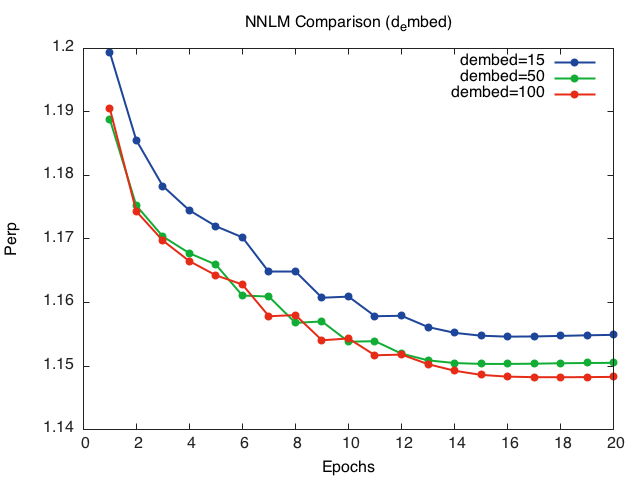
\includegraphics[width=12cm]{nnlmcompdwin.png}\\
    \textit{Figure 2: Comparing NNLMs of different $d_{win}$.}
\end{center}

\begin{center}
    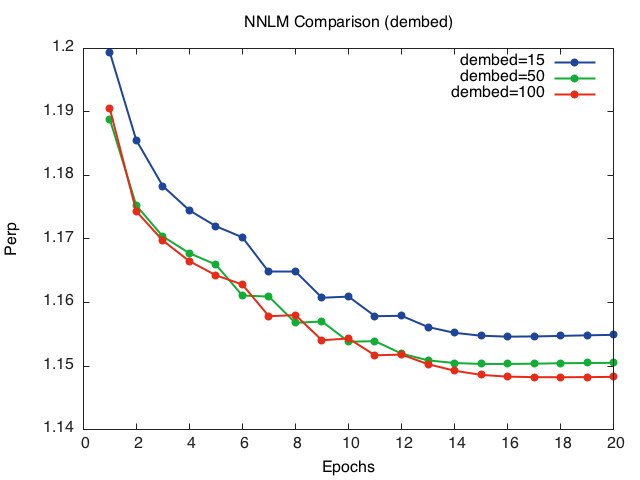
\includegraphics[width=12cm]{nnlmcompdembed.png}\\
    \textit{Figure 3: Comparing NNLMs of different $d_{embed}$.}
\end{center}

To further push the performance on the segmentation task, the cutoff threshold for predicting a space was selected based on performance on held-out validation examples. As the models tended to slightly under-predict, a cutoff of 0.4 was chosen (as opposed to the default 0.5).

\begin{table}[h]
\centering
\begin{tabular*}{0.75\textwidth}{@{\extracolsep{\fill} }| c | c | c | c |}
\toprule
Model & PTB (Train Perp) & PTB (Valid Perp) & PTB (Valid Seg MSE)\\
\midrule
\textsc{NNLM2} & 1.27 & 1.27 & 18.08\\
\textsc{NNLM4} & 1.14 & 1.16 & 7.24\\
\textsc{NNLM5} & 1.13 & 1.15 & 7.11\\
\textsc{NNLM6} & 1.13 & 1.15 & 6.90\\
\textsc{NNLM7} & 1.13 & 1.15 & 6.51\\
\textsc{NNLM9} & 1.13 & 1.15 & \textbf{6.15}\\
\textsc{NNLM11} & 1.13 & 1.15 & 6.80\\
\bottomrule
\end{tabular*}
\caption{\label{tab:results} Performance of NNLMs. Suffix numbers refer to $d_{win}$. $d_{embed}=50$.}
\end{table}

\subsection{RNNs}

During RNN experimentation, we mainly examined the effects of changing the embedding size $d_{embed}$, the recurrent unit structure (LSTM vs. GRU), and the model's topology (stacked LSTMs). As in training for NNLMs, the learning rate $\eta$ was initially set to 0.01, then dynamically modified during training to prevent stagnation. During experimentation, sequence length was held constant at 50. As expected, the RNN variants proved most adept out of all models at sequence modeling.

Surprisingly, the character embedding size $d_{embed}$ again did not affect performance much on the segmentation task, though it did affect the raw language modeling task. A comparison of embedding size effect on LSTM performance can be seen in \textit{Figure 4}. The highest performing model from all experiments was a two-layer LSTM with $d_{embed}=50$, trained on sequences of length 50 and with mini-batches of size 32. Interestingly, this model did not post the best perplexity but it did generalize very well to segmentation. We found that LSTM and GRU variants performed about equally on the language modeling task, though long short-term memory units outperform gated recurrent units slightly on the segmentation task.

\begin{center}
    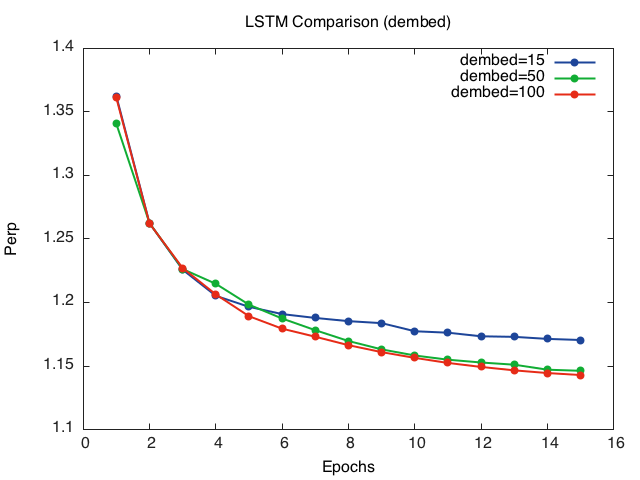
\includegraphics[width=12cm]{lstmcompdembed.png}\\
    \textit{Figure 4: Comparing LSTMs of different $d_{embed}$.}
\end{center}

\begin{table}[h]
\centering
\begin{tabular*}{0.85\textwidth}{@{\extracolsep{\fill} }| c | c | c | c |}
\toprule
Model & PTB (Train Perp) & PTB (Valid Perp) & PTB (Valid Seg MSE)\\
\midrule
\textsc{LSTM} & 1.12 & 1.14 & 5.90\\
\textsc{GRU} & 1.12 & 1.15 & 6.09\\
\textsc{Stack LSTM} & 1.16 & 1.17 & \textbf{5.81}\\
\bottomrule
\end{tabular*}
\caption{\label{tab:results} Performance of RNN variants.}
\end{table}

\section{Conclusion}

In conclusion, we were able to achieve solid results across our different models. Each class of models improved upon the last in the main segmentation task, with the highest performance posted by an LSTM variation influenced by \citet{DBLP:journals/neco/HochreiterS97}. Though the count-based and neural language models were able to achieve impressive performance on the training and validation metrics, especially with large n-gram values, this did not translate to segmentation performance in the way that RNNs exhibited.

The actual MSE scores achieved by our models were competitive on Kaggle, though still on average missed the correct number of spaces on each example by about 2. This performance might have been pushed even higher by more careful handling of the segmentation prediction structure: for example, the overall sequence could be broken into shorter sequences and recombined after prediction. Also, beam search would be an interesting alternative to greedy and Viterbi search for sequence selection during prediction. All code can be found on GitHub here \url{https://github.com/cgyulay/cs287/tree/master/HW4}, while Kaggle submissions can be found under the team name "Kid CUDA".

\bibliographystyle{apalike}
\bibliography{writeup}

\end{document}
